\documentclass[11pt]{article}
%Gummi|065|=)
%\title{\textbf{Welcome to Gummi 0.6.5}}

\title{\textbf{AIND Planning Project}}


 \renewcommand{\familydefault}{Hoefler}

\usepackage{amsmath}	
\usepackage{tikz}
\usepackage{xcolor}
\usepackage{float}
\usepackage{graphics}
\usepackage{graphicx}
\usepackage{wrapfig}
\usepackage{slashbox}
\usepackage{csvsimple}

\usetikzlibrary{shapes,arrows,chains}


\begin{document}

\maketitle

\newpage

\section{Uninformed Search}

%\begin{tabularx}{\linewidth}{llXX}\toprule %{|| c || c | c | c | c | c | c | c | c | c ||}\toprule

    %\bfseries algorithm & \bfseries p1 expansions & \bfseries p1 goal tests & \bfseries p1 new nodes & \bfseries p2 expansions & \bfseries p2 goal tests & \bfseries p2 new nodes & \bfseries p3 expansions & \bfseries p3 goal tests % specify table head
%    \textbf{A} & \textbf{B} & \textbf{C} & \textbf{D}\\\midrule
%    \csvreader[late after line=\\\midrule,late after last line=\\\bottomrule]{uninformed_results_summary_ls.csv}
    {}% use head of csv as column names
%    {\csvcoli &
    %\csvcolii & \csvcolii & \csvcolii &
    %\csvcolii & \csvcolii & \csvcolii & 
%    \csvcolii & \csvcolii & \csvcolii}% specify your coloumns here
%\end{tabularx}
\begin{figure}[h]
%	\centering
	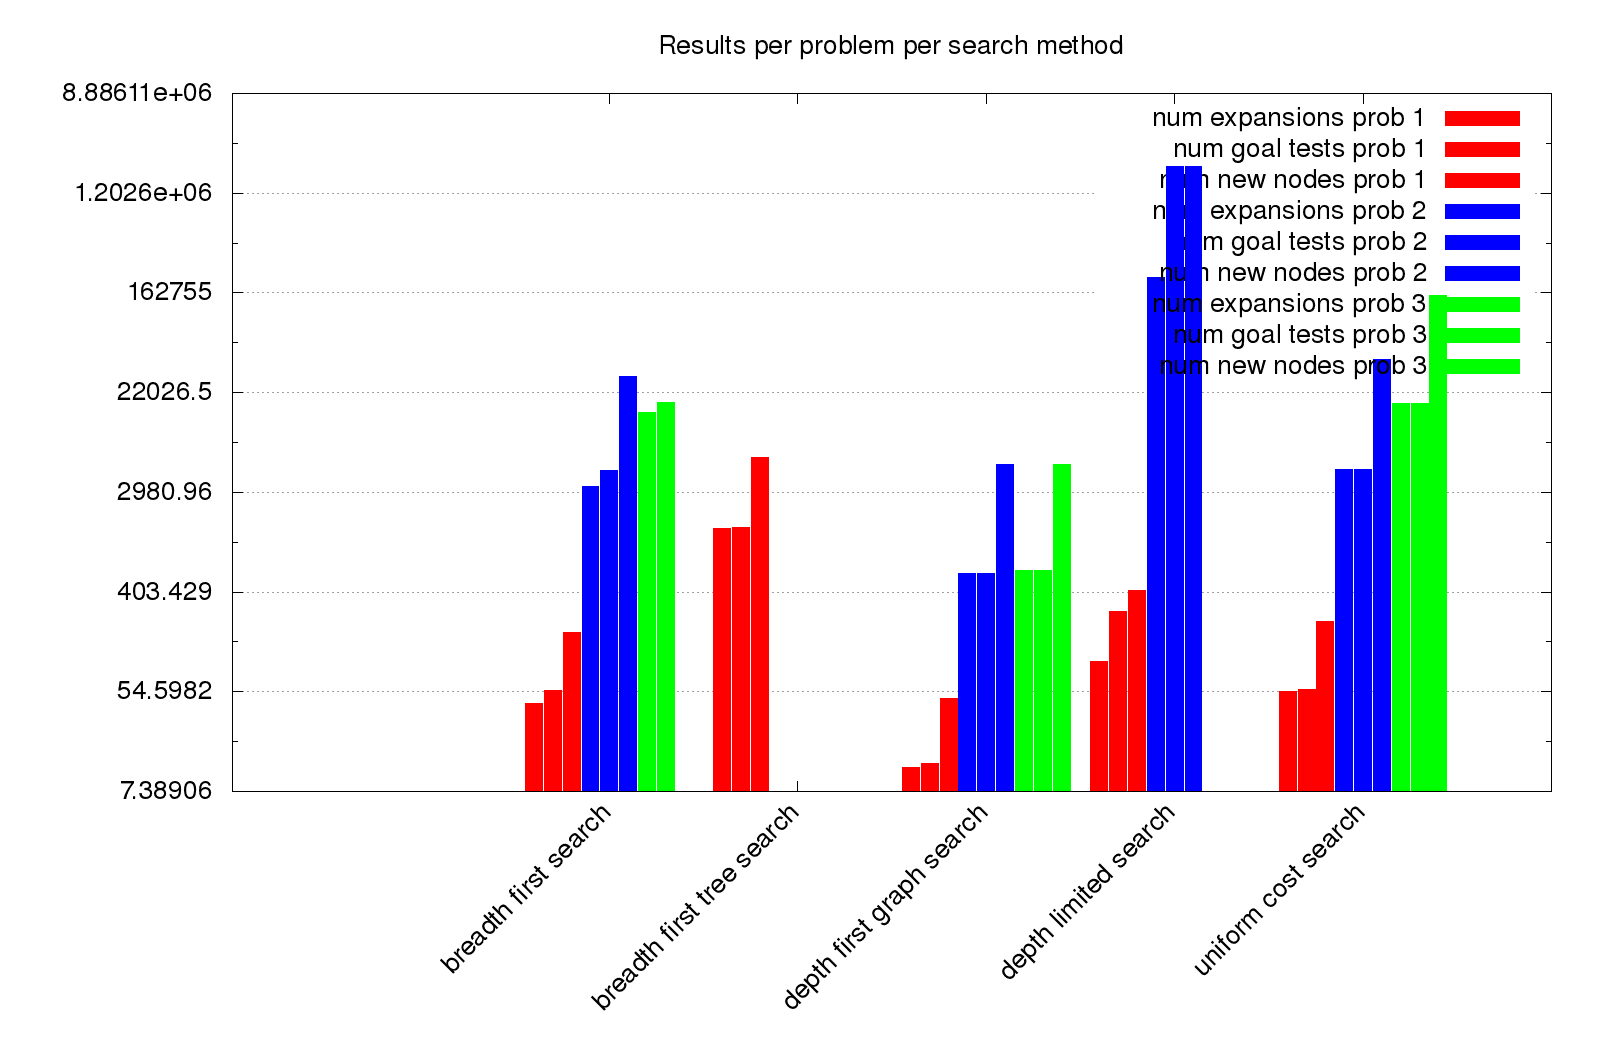
\includegraphics[scale=0.32]{results_summary.png}
	\caption{Results of each search method on each heuristic. The y axis is scaled to $log(e)$.
			 It should be noted that problems 2 and 3 were not solved by breadth first within reasonable time. and that problem 3 was not solved by depth limited in reasonable time.}
	\label{results}
\end{figure}

\begin{figure}
	\begin{tabular}{|p{2cm}|| p{1.3cm} p{1.3cm} p{1.3cm} p{1.3cm} p{1.3cm} p{1.3cm} p{1.3cm}|} 
		\hline
		algorithm & p1 num steps & p1 runtime & p2 num steps & p2 runtime & p3 num steps & p3 runtime \\
		\hline
		\hline
		breadth first search & 6 & 0.0227 & 9 & 10.3 & 12 & 80.6  \\
		\hline
		breadth first tree search & 6 & 0.680 & N/A & N/A & N/A & N/A  \\
		\hline
		depth first graph search & 12 & 0.00605 & 575 & 2.71 & 596 & 2.94  \\
		\hline
		depth limited search & 50 & 0.06507 & 50 & 730 & N/A & N/A  \\
		\hline
		uniform cost search & 6 & 0.0263 & 9 & 8.64 12 & 36.5  \\
		\hline
	\end{tabular}
	
\end{figure}

\subsection{Problem 1}
The simplest of problems with least goals and constraints

\subsection{Problem 2}

\subsection{Problem 3}



\end{document}
